
\documentclass{beamer}
\usecolortheme{dove}
\setbeamertemplate{navigation symbols}{}
\usepackage{amsmath,amssymb,amsfonts,amsthm, multicol, subfigure, color}
\usepackage{bm}
\usepackage{graphicx}
\usepackage{tabularx}
\usepackage{booktabs}
\usepackage{hyperref}
\usepackage{pdfpages}
\usepackage{xcolor}
\definecolor{seagreen}{RGB}{46, 139, 87}
\def\independenT#1#2{\mathrel{\rlap{$#1#2$}\mkern2mu{#1#2}}}
\newcommand\indep{\protect\mathpalette{\protect\independenT}{\perp}}
\def\log{\text{log}}
\newcommand\logit{\text{logit}}
\newcommand\iid{\stackrel{\text{iid}}{\sim}}
\newcommand\E{\text{E}}
\newcommand\V{\text{V}}
\renewcommand\P{\text{P}}
\newcommand{\Cov}{\text{Cov}}
\newcommand{\Cor}{\text{Cor}}
\newcommand\doop{\text{do}}
\usepackage{stackrel}
\usepackage{tikz}
\usetikzlibrary{arrows,shapes.arrows,positioning,shapes,patterns,calc}
\newcommand\slideref[1]{\vskip .1cm \tiny \textcolor{gray}{{#1}}}
\newcommand\red[1]{\color{red}#1}
\newcommand\blue[1]{\color{blue}#1}
\newcommand\gray[1]{\color{gray}#1}
\newcommand\seagreen[1]{\color{seagreen}#1}
\newcommand\purple[1]{\color{purple}#1}
\newcommand\orange[1]{\color{orange}#1}
\newcommand\black[1]{\color{black}#1}
\newcommand\white[1]{\color{white}#1}
\newcommand\teal[1]{\color{teal}#1}
\newcommand\magenta[1]{\color{magenta}#1}
\newcommand\Fuchsia[1]{\color{Fuchsia}#1}
\newcommand\BlueGreen[1]{\color{BlueGreen}#1}
\newcommand\bblue[1]{\textcolor{blue}{\textbf{#1}}}
\newcommand\bred[1]{\textcolor{red}{\textbf{#1}}}
\newcommand\bgray[1]{\textcolor{gray}{\textbf{#1}}}
\newcommand\bgreen[1]{\textcolor{seagreen}{\textbf{#1}}}
\newcommand\bref[2]{\href{#1}{\color{blue}{#2}}}
\colorlet{lightgray}{gray!40}
\pgfdeclarelayer{bg}    % declare background layer for tikz
\pgfsetlayers{bg,main} % order layers for tikz
\newcommand\mycite[1]{\begin{scriptsize}\textcolor{darkgray}{(#1)}\end{scriptsize}}
\newcommand{\tcframe}{\frame{
%\small{
\only<1|handout:0>{\tableofcontents}
\only<2|handout:1>{\tableofcontents[currentsection]}}
%}
}

\usepackage[round]{natbib}
\bibliographystyle{humannat-mod}
\setbeamertemplate{enumerate items}[default]
\usepackage{mathtools}

\newcommand{\goalsframe}{\begin{frame}{Learning goals for today}
At the end of class, you will be able to estimate average causal effects by modeling treatment assignment probabilities. \vskip .2in
Optional reading:
\begin{itemize}
\item Hernán and Robins 2020 Chapter 12.1--12.5, 13, 15.1
\end{itemize}
\end{frame}}

\title{Model-based causal estimation:\\From outcome models to treatment weighting}
\author{Ian Lundberg\\Sociol 114\\\bref{https://soc114.github.io/}{soc114.github.io}}
\date{Winter 2025}

\begin{document}

\maketitle

\goalsframe


\begin{frame}{Review of what we have learned}

Causal assumptions
\begin{center}
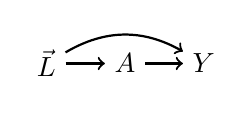
\begin{tikzpicture}
\node (l) at (0,0) {$\vec{L}$};
\node (a) at (1,0) {$A$};
\node (y) at (2,0) {$Y$};
\draw[->, thick] (l) -- (a);
\draw[->, thick] (a) -- (y);
\draw[->, thick] (l) to[bend left] (y);
\end{tikzpicture}
\end{center} \pause

Nonparametric estimator
\begin{itemize}
\item Group by $L$, then mean difference in $Y$ over $A$
\item Re-aggregate over subgroups
\end{itemize} \vskip .1in \pause

Outcome modeling estimator
\begin{itemize}
\item Model $Y^1$ given $L$ among the treated
\item Model $Y^0$ given $L$ among the untreated
\item Predict for everyone and take the difference
\item Average over all units
\end{itemize}

\end{frame}

\begin{frame}{Inverse probability of treatment weighting}


\begin{tikzpicture}[x = \textwidth, y = .8\textheight]
\node at (0,0) {};
\node at (1,1) {};
\node[anchor = north] at (.45,.9) {$L = 0$};
\node[anchor = north] at (.85,.9) {$L = 1$};
\only<1-3>{
\draw[rounded corners] (.3,.4) rectangle (.6,1);
\draw[rounded corners] (.7,.4) rectangle (1,1);
}
\only<4->{
\draw[dashed, rounded corners] (.3,.4) rectangle (.6,1);
\draw[dashed, rounded corners] (.7,.4) rectangle (1,1);
}
\node[anchor = north west, gray, font = \Huge] (unsamp) at (0,.9) {$\bullet$};
\node[anchor = west, gray] at (unsamp.east) {Untreated};
\node[anchor = north west, blue, font = \Huge] (samp) at (unsamp.south west) {$\bullet$};
\node[anchor = west, blue] (samp.east) at (samp.east) {Treated};
% L = 0
\node[gray, font = \Huge] at (.4,.6) {$\bullet$};
\node[blue, font = \Huge] at (.5,.5) {$\bullet$};
\node[gray, font = \Huge] at (.55,.45) {$\bullet$};
\node[gray, font = \Huge] at (.45,.7) {$\bullet$};
\only<4->{
\node[gray, font = \small, anchor = south, outer sep = 4pt] at (.4,.6) {4/3};
\node[blue, font = \small, anchor = south, outer sep = 4pt] at (.5,.5) {4};
\node[gray, font = \small, anchor = south, outer sep = 4pt] at (.55,.45) {4/3};
\node[gray, font = \small, anchor = south, outer sep = 4pt] at (.45,.7) {4/3};
}
% L = 1
\node[blue, font = \Huge] at (.75,.52) {$\bullet$};
\node[blue, font = \Huge] at (.85,.44) {$\bullet$};
\node[blue, font = \Huge] at (.95,.63) {$\bullet$};
\node[gray, font = \Huge] at (.9,.72) {$\bullet$};
\only<4->{
\node[blue, font = \small, anchor = south, outer sep = 4pt] at (.75,.52) {4/3};
\node[blue, font = \small, anchor = south, outer sep = 4pt] at (.85,.44) {4/3};
\node[blue, font = \small, anchor = south, outer sep = 4pt] at (.95,.63) {4/3};
\node[gray, font = \small, anchor = south, outer sep = 4pt] at (.9,.72) {4};
}
% P(S)
\node<2->[anchor = east, font = \large] at (.45,.2) {Propensity score:};
\node<2->[anchor = west, font = \large] at (.5,.2) {$\pi_i = \P(A = A_i\mid L = L_i)$};
\node<3->[anchor = east, font = \large] at (.45,.1) {Inverse probability weight:};
\node<3->[anchor = west, font = \large] at (.5,.1) {$w_i = \frac{1}{\pi_i}$};
\only<5->{
\node[anchor = west, align = left, font = \footnotesize] at (0.01,.6) {pseudo-population};
\node[font = \small] (l) at (.03,.5) {$L$};
\node[font = \small] (a) at (.13,.5) {$A$};
\node[font = \small] (y) at (.23,.5) {$Y$};
\draw[->, thick] (a) -- (y);
\draw[->, thick] (l) to[bend left] (y);
\draw[dashed, rounded corners] (.01,.45) rectangle (.27,.65);
}
\end{tikzpicture}

\end{frame}

\begin{frame}

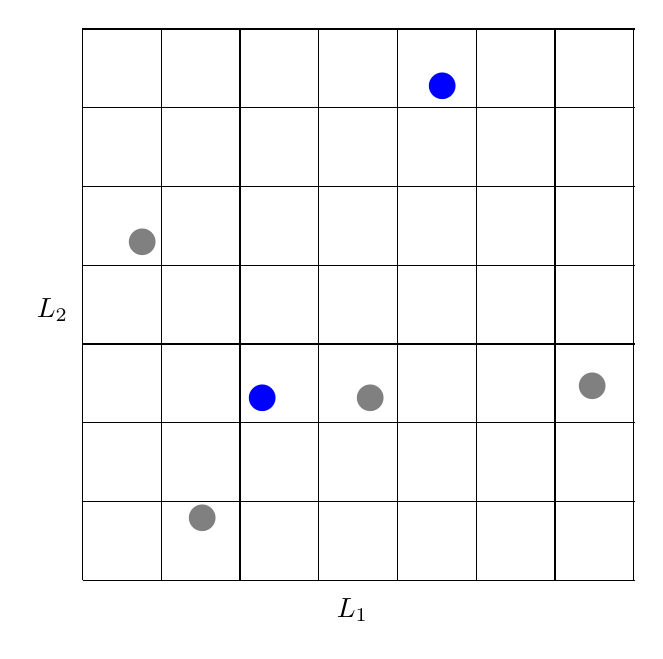
\begin{tikzpicture}[x = .3in, y = .3in]
\node at (4.5,-.5) {$L_1$};
\node at (-.5,4.5) {$L_2$};
\draw (0,0) grid (9.2,9.2);
\node[gray, font = \Huge] at (1,5.6) {$\bullet$};
\node[gray, font = \Huge] at (2,1) {$\bullet$};
\node[blue, font = \Huge] at (3,3) {$\bullet$};
\node[gray, font = \Huge] at (4.8,3) {$\bullet$};
\node[blue, font = \Huge] at (6,8.2) {$\bullet$};
\node[gray, font = \Huge] at (8.5,3.2) {$\bullet$};
\end{tikzpicture}

\end{frame}

\begin{frame}

\bgray{Model} the treatment assignment

$$\begin{aligned}
\hat\P(A = 1\mid \vec{L}) &= \logit^{-1}\left(\hat\alpha + \hat{\vec\gamma}\vec{L}\right)
\end{aligned}
$$

\bgray{Predict} the propensity score for each unit

$$\begin{aligned}
\hat\pi_i &= \begin{cases}
\logit^{-1}\left(\hat\alpha + \hat{\vec\gamma}\vec{L}\right) &\text{if }A_i=1 \\
1 - \logit^{-1}\left(\hat\alpha + \hat{\vec\gamma}\vec{L}\right) &\text{if }A_i=0 \\
\end{cases}
\end{aligned}$$

\bgray{Estimate} by inverse probability weighting

$$\begin{aligned}
\hat\E(Y^a) &= \frac{1}{N}\sum_{i:A_i=a}\frac{Y_i}{\hat\pi_i}
\end{aligned}$$

\end{frame}

\begin{frame}
Visual summaries: Two strategies
\end{frame}

\begin{frame}{A visual summary of outcome modeling}
\begin{center}
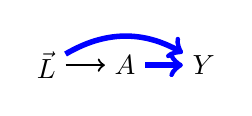
\begin{tikzpicture}
\node (l) at (0,0) {$\vec{L}$};
\node (a) at (1,0) {$A$};
\node (y) at (2,0) {$Y$};
\draw[->, thick] (l) -- (a);
\draw[->, thick, line width = 2pt, blue] (a) -- (y);
\draw[->, thick, line width = 2pt, blue] (l) to[bend left] (y);
\end{tikzpicture}
\end{center}
Predict outcomes under treatment and control
\end{frame}

\begin{frame}{A visual summary of treatment weighting}
\begin{center}
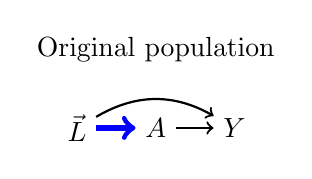
\begin{tikzpicture}
\node at (1,1) {Original population};
\node (l) at (0,0) {$\vec{L}$};
\node (a) at (1,0) {$A$};
\node (y) at (2,0) {$Y$};
\draw[->, line width = 2pt, blue] (l) -- (a);
\draw[->, thick] (a) -- (y);
\draw[->, thick] (l) to[bend left] (y);
\end{tikzpicture}
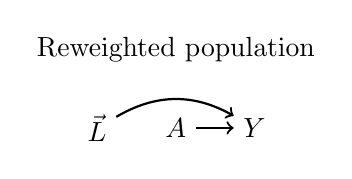
\begin{tikzpicture}
\node at (1,1) {Reweighted population};
\node (l) at (0,0) {$\vec{L}$};
\node (a) at (1,0) {$A$};
\node (y) at (2,0) {$Y$};
\draw[->, thick] (a) -- (y);
\draw[->, thick] (l) to[bend left] (y);
\end{tikzpicture}
\end{center}
Re-weight to a pseudo-population in which $A$ does not depend on $\vec{L}$
\end{frame}

\goalsframe

\begin{frame}{Problem: Extreme weights create high variance}

\pause
Suppose a stratum $\vec{L} = \vec\ell$ contains
\begin{itemize}
\item 100 untreated units
\item 1 treated unit
\end{itemize} \pause
The treated unit gets a weight of 100.\vskip .2in \pause
The estimate depends heavily on which treated unit happens to be included in the sample $\rightarrow$ high-variance estimator \vskip .2in \pause
Two solutions
\begin{enumerate}
\item Trim the weights
\item Truncate the weights
\end{enumerate} \pause
Both solutions accept bias in order to reduce variance

\end{frame}

\begin{frame}{Accepting bias to reduce variance: Trimming}

\begin{tikzpicture}[x = \textwidth, y = .8\textheight]
\node at (0,0) {};
\node at (1,1) {};
\node<1>[anchor = west] at (0,.5) {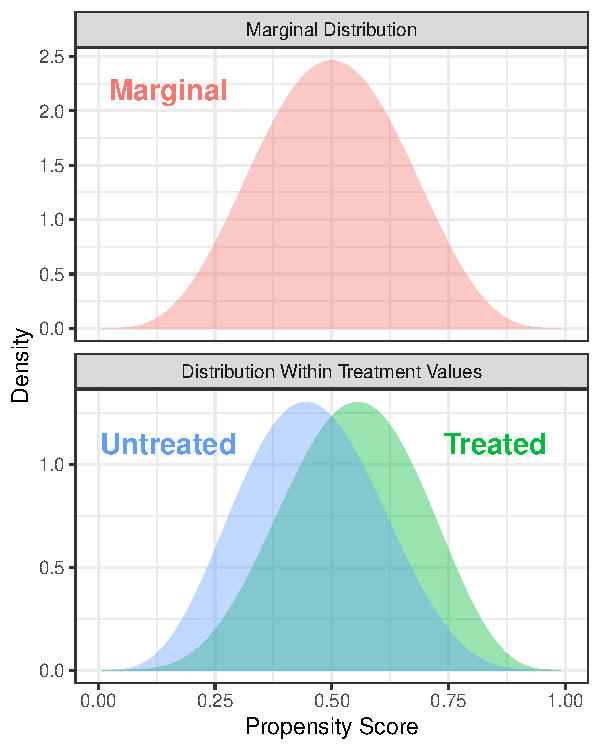
\includegraphics[height = .8\textheight]{figures/propensity_overlap}};
\node<2-3>[anchor = west] at (0,.5) {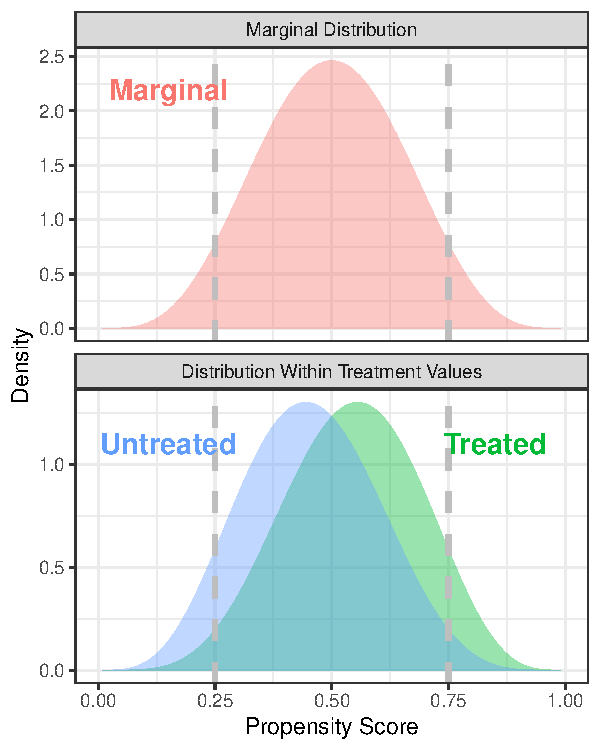
\includegraphics[height = .8\textheight]{figures/propensity_overlap_1}};
\node<3->[anchor = west, align = left] at (.6,.7) {Drop units with\\extreme weights};
\node<4->[anchor = west] at (0,.5) {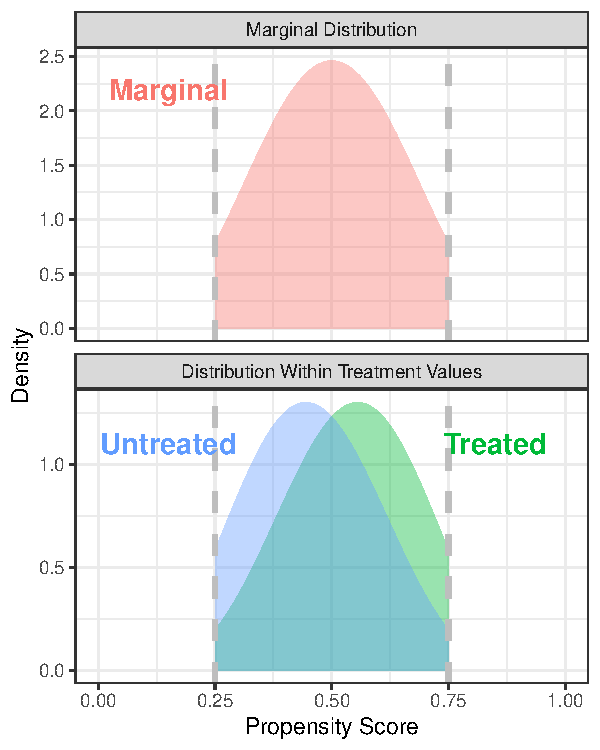
\includegraphics[height = .8\textheight]{figures/propensity_overlap_trim}};
\node<5->[anchor = west, align = left] at (.6,.5) {Changes target population\\--- Biased for full population};
\end{tikzpicture}

\end{frame}

\begin{frame}{Accepting bias to reduce variance: Weight truncation}

\begin{tikzpicture}[x = \textwidth, y = .8\textheight]
\node at (0,0) {};
\node at (1,1) {};
\node<1-2>[anchor = west] at (0,.5) {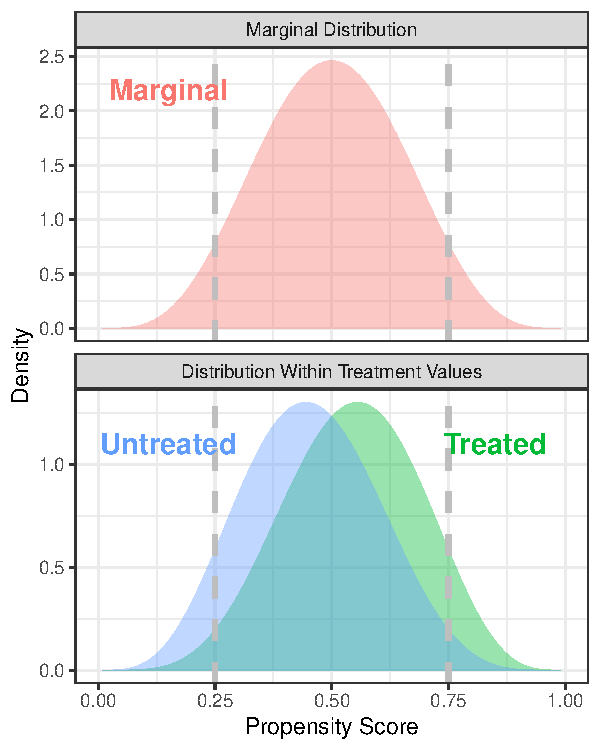
\includegraphics[height = .8\textheight]{figures/propensity_overlap_1}};
\node<2->[anchor = west, align = left] at (.6,.7) {Truncate values of\\extreme weights};
\node<3->[anchor = west] at (0,.5) {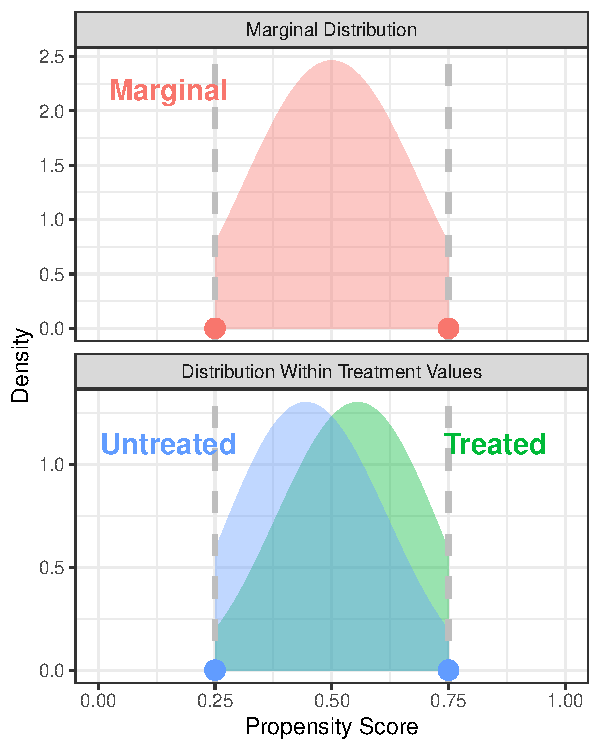
\includegraphics[height = .8\textheight]{figures/propensity_overlap_truncate}};
\node<4->[anchor = west, align = left] at (.6,.5) {Biased: Ignores\\some confounding};
\end{tikzpicture}

\end{frame}

\goalsframe


\end{document}














% OUTTAKES

\begin{frame}{The parametric g-formula: Connection to $\hat\beta$} \pause
Estimator for the effect $\E(Y^1) - \E(Y^0)$: \pause
$$\begin{aligned}
\hat\E(Y^1) - \hat\E(Y^0) 
&= \left(\frac{1}{n}\sum_{i=1}^n \bigg(\hat\alpha + \hat\gamma \ell_i + \hat\beta \times 1\bigg)\right) \\
&\qquad - \left(\frac{1}{n}\sum_{i=1}^n \bigg(\hat\alpha + \hat\gamma \ell_i + \hat\beta \times 0\bigg)\right) \\ \pause
&= \frac{1}{n}\sum_{i=1}^n \hat\beta \\ \pause
&= \hat\beta
\end{aligned}$$ \pause
With OLS, the parametric g-formula collapses on the coefficient.
\end{frame}

\begin{frame}{The parametric g-formula is more general}
Suppose the effect of $A$ depends on $L$
$$\E(Y\mid A, L) = \alpha + \gamma L + \beta A + \eta AL$$ \pause
Estimator for the effect $\E(Y^1) - \E(Y^0)$:
$$\begin{aligned}
\hat\E(Y^1) - \hat\E(Y^0) 
&= \left(\frac{1}{n}\sum_{i=1}^n \bigg(\hat\alpha + \hat\gamma \ell_i + \hat\beta \times 1 + \hat\eta \times  1\times \ell_i)\bigg) \right) \\
&\qquad - \left(\frac{1}{n}\sum_{i=1}^n \bigg(\hat\alpha + \hat\gamma \ell_i + \hat\beta \times 0 + \hat\eta\times 0 \times \ell_i\bigg) \right) \\ \pause
&= \frac{1}{n}\sum_{i=1}^n \left(\hat\beta + \hat\eta \ell_i\right)
\end{aligned}$$
The g-formula no longer collapses to a coefficient!
\end{frame}

\begin{frame}{Parametric g-formula: Outcome model recap}

\begin{center}
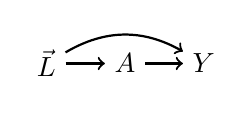
\begin{tikzpicture}
\node (l) at (0,0) {$\vec{L}$};
\node (a) at (1,0) {$A$};
\node (y) at (2,0) {$Y$};
\draw[->, thick] (l) -- (a);
\draw[->, thick] (a) -- (y);
\draw[->, thick] (l) to[bend left] (y);
\end{tikzpicture}
\end{center}

\begin{enumerate}
\item Model the outcome mean $\E(Y\mid A,\vec{L})$
\item Change everyone's treatment to the value of interest
\item Predict for everyone
\item Take the average
\end{enumerate}
$$\hat\E(Y^a) = \frac{1}{n}\sum_{i=1}^n \hat\E(Y\mid \vec{L} = \vec\ell_i, A = a)$$

\end{frame}



\begin{frame}{Nonparametric estimation breaks down}
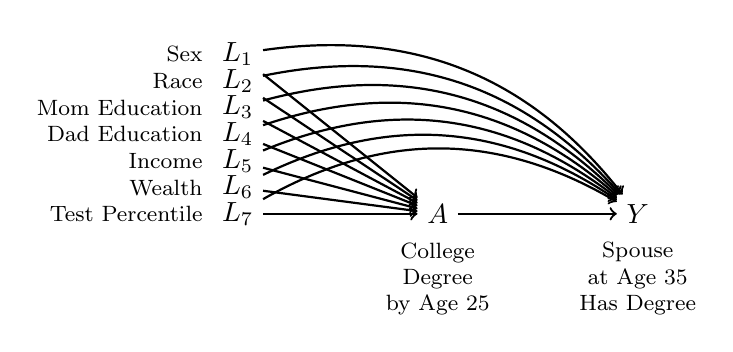
\begin{tikzpicture}[x = 1in, y = .4in]
\node (a) at (0,0) {$A$};
\node (y) at (1,0) {$Y$};
\node (l1) at (-1,2) {$L_1$};
\node (l2) at (-1,1.66) {$L_2$};
\node (l3) at (-1,1.33) {$L_3$};
\node (l4) at (-1,1) {$L_4$};
\node (l5) at (-1,.66) {$L_5$};
\node (l6) at (-1,.33) {$L_6$};
\node (l7) at (-1,0) {$L_7$};
\draw[->, thick] (l1) -- (a);
\draw[->, thick] (l2) -- (a);
\draw[->, thick] (l3) -- (a);
\draw[->, thick] (l4) -- (a);
\draw[->, thick] (l5) -- (a);
\draw[->, thick] (l6) -- (a);
\draw[->, thick] (l7) -- (a);
\draw[->, thick] (a) -- (y);
\draw[->, thick] (l1) to[bend left] (y);
\draw[->, thick] (l2) to[bend left] (y);
\draw[->, thick] (l3) to[bend left] (y);
\draw[->, thick] (l4) to[bend left] (y);
\draw[->, thick] (l5) to[bend left] (y);
\draw[->, thick] (l6) to[bend left] (y);
\draw[->, thick] (l7) to[bend left] (y);
\node[anchor = north, align = center, font = \footnotesize] at (a.south) {College\\Degree\\by Age 25};
\node[anchor = north, align = center, font = \footnotesize] at (y.south) {Spouse\\at Age 35\\Has Degree};
\node[anchor = east, align = center, font = \footnotesize] at (l1.west) {Sex};
\node[anchor = east, align = center, font = \footnotesize] at (l2.west) {Race};
\node[anchor = east, align = center, font = \footnotesize] at (l3.west) {Mom Education};
\node[anchor = east, align = center, font = \footnotesize] at (l4.west) {Dad Education};
\node[anchor = east, align = center, font = \footnotesize] at (l5.west) {Income};
\node[anchor = east, align = center, font = \footnotesize] at (l6.west) {Wealth};
\node[anchor = east, align = center, font = \footnotesize] at (l7.west) {Test Percentile};
\end{tikzpicture}
\end{frame}

\begin{frame}{Nonparametric estimation breaks down}
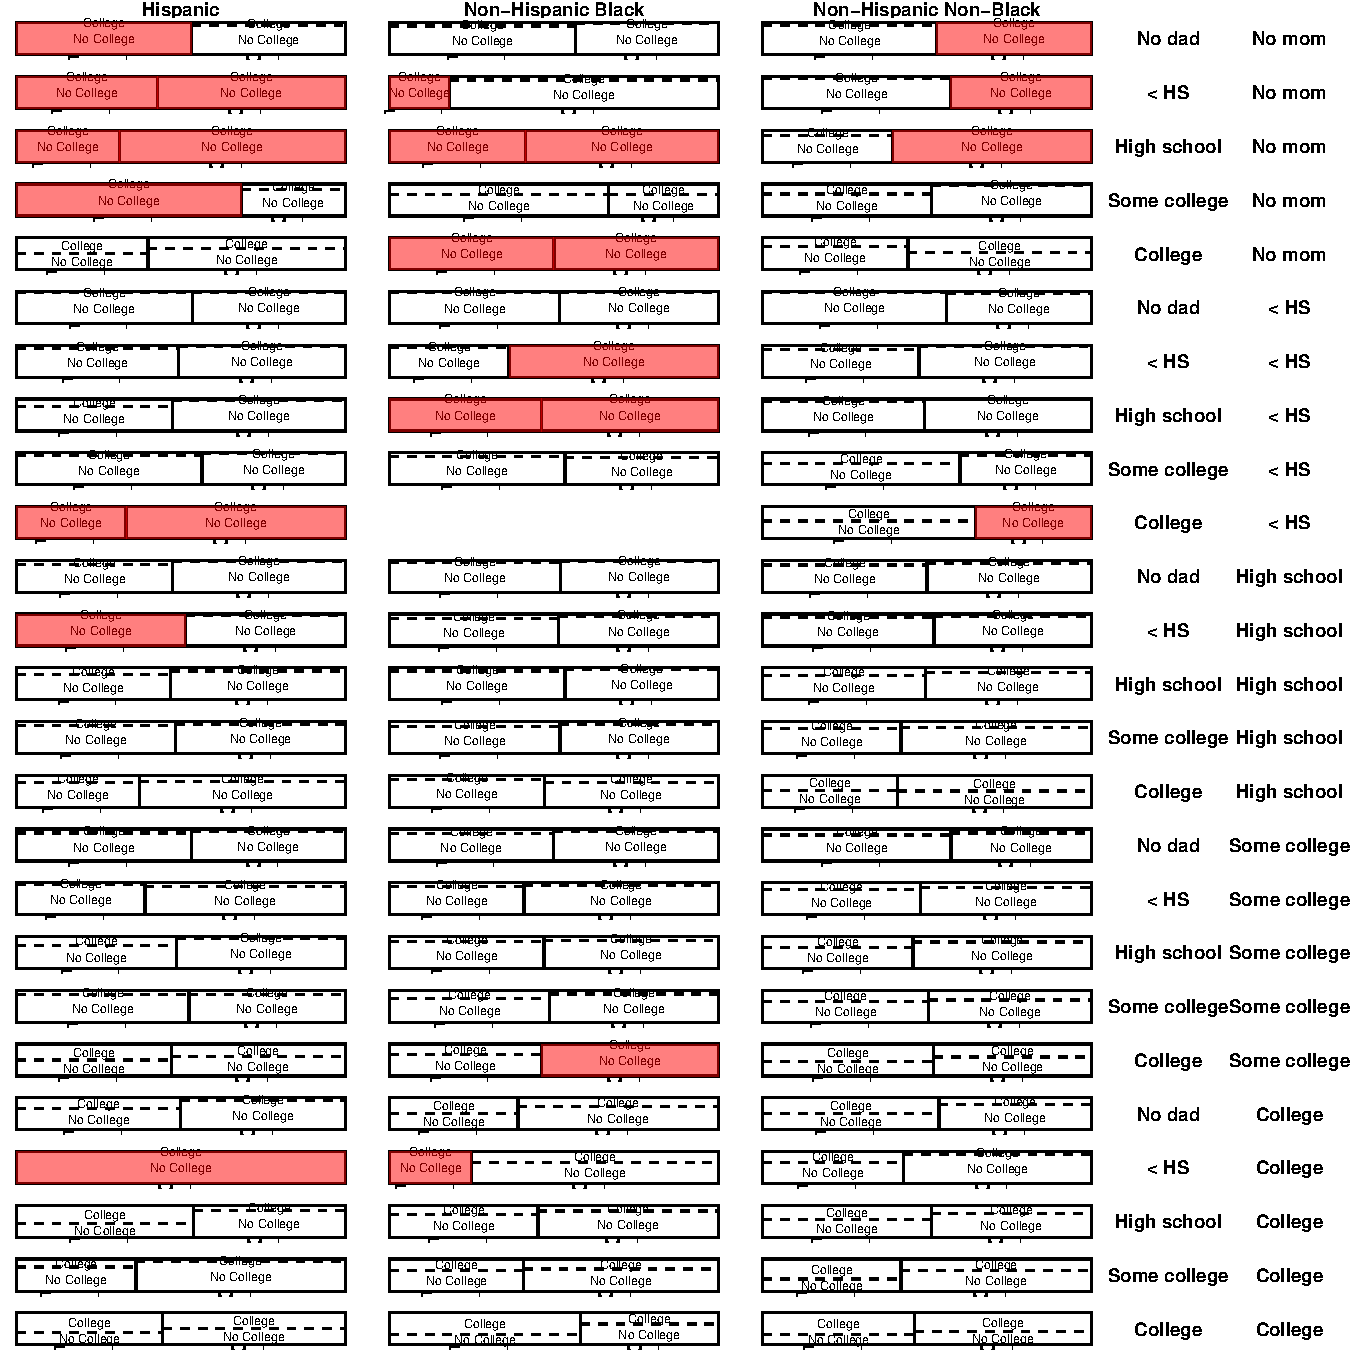
\includegraphics[width = .7\textwidth]{figures/curse}
\end{frame}

\begin{frame}{Parametric estimation: Outcome model}

Causal assumptions
\begin{center}
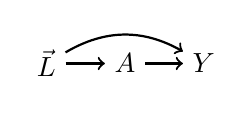
\begin{tikzpicture}
\node (l) at (0,0) {$\vec{L}$};
\node (a) at (1,0) {$A$};
\node (y) at (2,0) {$Y$};
\draw[->, thick] (l) -- (a);
\draw[->, thick] (a) -- (y);
\draw[->, thick] (l) to[bend left] (y);
\end{tikzpicture}
\end{center}

Parametric estimator
$$\begin{aligned}
\hat\E(Y^a) &= \frac{1}{n}\sum_{i=1}^n \hat\E(Y\mid \vec{L} = \vec\ell_i, A = a)
\end{aligned}$$ \pause

Where $\hat{E}$ is a model-based prediction
$$\hat\E(Y\mid \vec{L}, A) = \hat\alpha + \vec{L}'\hat{\vec\gamma} + A\hat\beta$$ \pause

\end{frame}